%%%%%%%%%%%%%%%%%%%%%%%%%%%%%%%%%%%%%%%%%%%%%%%%%%%%%%%%%%%%%%%%%%%%%%%%%%%%%%%%
%%
%%   BornAgain User Manual
%%
%%   homepage:   http://www.bornagainproject.org
%%
%%   copyright:  Forschungszentrum Jülich GmbH 2015
%%
%%   license:    Creative Commons CC-BY-SA
%%   
%%   authors:    Scientific Computing Group at MLZ Garching
%%               C. Durniak, M. Ganeva, G. Pospelov, W. Van Herck, J. Wuttke
%%
%%%%%%%%%%%%%%%%%%%%%%%%%%%%%%%%%%%%%%%%%%%%%%%%%%%%%%%%%%%%%%%%%%%%%%%%%%%%%%%%

\chapter{Foundations of GISAS}  \label{sec:ScatTheory}

In this chapter,
we present the theory
of grazing-incidence small-angle scattering (GISAS)
that underlies the simulation algorithm implemented in \BornAgain.
We specifically consider the propagation and scattering
of neutrons with no polarization-dependent interactions,
so that we can base our exposition on a scalar wave equation.
The notationally more involved
vectorial theory needed for X-rays and for polarized neutrons
is adjourned to the next chapter.

Our exposition is largely self-contained,
except for the initial passage from the microscopic
to the macroscopic Schrödinger equation,
which we outline only briefly.
This manual is decidedly not the place for renarrating
the historic development of GISAS theory.
For ample references to the original literature,
we refer to the excellent review \cite{ReLL09}.


%%%%%%%%%%%%%%%%%%%%%%%%%%%%%%%%%%%%%%%%%%%%%%%%%%%%%%%%%%%%%%%%%%%%%%%%%%%%%%%%
\section{Coherent neutron propagation}\label{Swave}
%%%%%%%%%%%%%%%%%%%%%%%%%%%%%%%%%%%%%%%%%%%%%%%%%%%%%%%%%%%%%%%%%%%%%%%%%%%%%%%%
\index{Wave propagation!neutrons|(}%
\index{Neutrons!wave propagation|(}%

\index{Schrodinger@Schrödinger equation!microscopic}%
The scalar wavefunction $\psi(\r,t)$
\nomenclature[2t020]{$t$}{Time}%
\nomenclature[2r040]{$\r$}{Position}%
\nomenclature[1ψ030 2r040 2t02]{$\psi(\r,t)$}{Microscopic neutron wavefunction}%
of a free neutron
is governed by the microscopic Schrödinger equation
\begin{equation}\label{ESchrodi}
  i\hbar\partial_t \psi(\r,t)
  = \left\{-\frac{\hbar^2}{2m}\Nabla^2+V(\r)\right\} \psi(\r,t).
\end{equation}
By assuming a time-independent potential $V(\r)$,
we have excluded inelastic scattering.
Therefore we only need to consider monochromatic waves
with given frequency~$\omega$.
\nomenclature[1ω 020]{$\omega$}{Frequency of incident radiation}%
In consequence, we have a stationary wavefunction
\begin{equation}\label{Estationarywave}
  \psi(\r,t) = \psi(\r)\e^{-i\omega t}.
\end{equation}
\nomenclature[1ψ030 2r040 0]{$\psi(\r)$}{Stationary wavefunction}%
The minus sign in the exponent of the phase factor
is an inevitable consequence of the standard form of the Schrödinger equation,
and is therefore called the \textit{quantum-mechanical sign convention}.
It is also used in most optics textbooks.
\index{Wave propagation|seealso {Sign convention}}%
\index{Sign convention}%
The opposite choice of a phase factor $\e^{+i\omega t}$ is 
called the \textit{crystallographic sign convention},
and is used in much of the literature on X-ray scattering,
including some important texts on GISAXS (e.~g.\ \cite{ReLL09}).
Since we are concerned with both X-rays and neutrons,
we had to make a somewhat arbitrary choice:

\Note
{\indent In this manual, and in the program code of \BornAgain,
the quantum-mechanical sign convention~(\ref{Estationarywave}) is chosen.
This has implications for the sign of the imaginary part of the
refractive index,
\index{Index of refraction|see {Refractive index}}
\index{Refractive index!sign convention}%
as explained in Sect.~\ref{Sabsorption}.}

Inserting (\ref{Estationarywave}) in (\ref{ESchrodi}),
we obtain the stationary Schrödinger equation
\begin{equation}\label{EstatSchrodi}
  \left\{-\frac{\hbar^2}{2m}\Nabla^2+V(\r)-\hbar\omega\right\} \psi(\r) = 0.
\end{equation}
\nomenclature[2m020]{$m$}{Neutron mass}%
\nomenclature[2v130 2r040]{$V(\r)$}{Microscopic optical potential}%
\index{Potential|see {Optical potential}}%
\index{Optical potential!nuclear (microscopic)}%
The \textit{nuclear} (or \textit{microscopic})
\textit{optical potential} $V(\r)$,
in a somewhat ``naive conception'' \cite[p.~7]{Sea89},
consists of a sum of delta functions,
representing Fermi's ``pseudopotential''.
\index{Fermi's pseudopotential}%
The superposition of the incident wave with the scattered waves
originating from each illuminated nucleus
results in \textit{coherent forward scattering},
\index{Coherent forward scattering}%
in line with Huygens' principle.
\index{Huygens' principle}%

Coherent superposition also leads to \textit{Bragg scattering}.
\index{Bragg scattering!by atomic lattices}%
However, Bragg scattering by atomic lattices only occurs at angles
far above the small-angle range covered in GISAS experiments.
Accordingly, it can be neglected in the analysis of GISAS data,
or at most, is taken into account as a loss channel.

Therefore,
we can neglect the atomic structure of $V(\r)$,
and perform some coarse graining to
arrive at a \textit{continuum approximation}.
\index{Continuum approximation!neutron propagation}%
This is 
similar to the passage from
the microscopic to the macroscopic Maxwell equations.
The details are intricate \cite{Sea89,Lax51},
but the result \cite[eq.~2.8.32]{Sea89} looks very simple:
The macroscopic field equation
has still the form of a stationary Schrödinger equation,
\index{Schrodinger@Schrödinger equation!macroscopic}%
\begin{equation}\label{EmacrSchrodi}
  \left\{-\frac{\hbar^2}{2m}\Nabla^2+v(\r)-\hbar\omega\right\} \psi(\r) = 0,
\end{equation}
\nomenclature[1ψ030 2r040 2t020]{$\psi(\r,t)$}{Coherent wavefunction}%
\nomenclature[2v020 2r040]{$v(\r)$}{Macrosopic optical potential}%
where $\psi$ now stands for the \textit{coherent wavefunction}
\index{Coherent wavefunction}%
\index{Wave propagation!coherent}%
obtained by superposition of
incident and forward scattered states,
and $v(\r)$ is the \textit{macroscopic optical potential}.
\index{Optical potential!macroscopic}%
This potential is weak, and slowly varying compared to atomic length scales.
It can be rewritten in a number of ways,
especially in terms of a
\textit{bound scattering length density}
\index{Scattering length density}%
$\rho_s(\r)$ \cite[eq.\ 2.8.37]{Sea89},
\nomenclature[1ρ 034 2s000 2r040]{$\rho_s(\r)$}{Scattering length density}%
\begin{equation}
  v(\r)=\frac{2\pi \hbar^2}{m}\rho_s(\r),  
\end{equation}
or of a \textit{refractive index}~$n(\r)$
\nomenclature[2n020 2r040]{$n(\r)$}{Refractive index}%
\index{Refractive index} % !vs scattering length density}%
\index{Index of refraction|see {Refractive index}}%
defined by
\begin{equation}\label{EnRefrIndx}
  n(\r)^2\coloneqq 1-\frac{4\pi}{K^2}\rho_s(\r) = 1 -\frac{2m}{\hbar^2 K^2}v(\r).
\end{equation}
In the latter expression,
we introduced the \textit{vacuum wavenumber}~$K$,
\nomenclature[2k120]{$K$}{Vacuum wavenumber, corresponding to the frequency~$\omega$}%
which is connected with the frequency~$\omega$ through the
\textit{dispersion relation}
\begin{equation}
  \frac{\hbar^2 K^2}{2m} = \hbar\omega.
\end{equation}
Since we only consider stationary solutions~(\ref{Estationarywave}),
$\omega$ will not appear any further in our derivations.
Instead, we use~$K$ as the given parameter that characterizes the
incoming radiation.
In terms of $K$ and $n$,
the macroscopic Schrödinger equation (\ref{EmacrSchrodi})
can be rewritten as
\Emph{
\begin{equation}\label{EnSchrodi}
  \left\{\Nabla^2+K^2n(\r)^2\right\}\psi(\r) = 0.
\end{equation}\vspace*{-10pt}
}
This equation is the starting point for the analysis of all
small-angle scattering experiments,
whether under grazing incidence (GISAS) or not (regular SAS).
\index{SAS|see {Small-angle scattering}}%
\index{Small-angle scattering}%

\index{Wave propagation!neutrons|)}%
\index{Neutrons!wave propagation|)}%

%%%%%%%%%%%%%%%%%%%%%%%%%%%%%%%%%%%%%%%%%%%%%%%%%%%%%%%%%%%%%%%%%%%%%%%%%%%%%%%%
\section{Neutron scattering in Born approximation}
%%%%%%%%%%%%%%%%%%%%%%%%%%%%%%%%%%%%%%%%%%%%%%%%%%%%%%%%%%%%%%%%%%%%%%%%%%%%%%%%

%===============================================================================
\subsection{The Born expansion}\label{SBorn}
%===============================================================================

\index{Born approximation|(}%

To describe an elastic scattering experiment,
we need to solve the Schrödinger equation~(\ref{EnSchrodi})
under the asymptotic boundary condition
\begin{equation}\label{Escabouco}
  \psi(\r)
  \to \psi_\ti(\r) + f(\vartheta,\varphi)\frac{\e^{iKr}}{4\pi r}
  \text{~for~}r\to\infty,
\end{equation}
\nomenclature[1ψ034 2i000 2r040]{$\psi_\ti(\r)$}{Incident wavefunction}%
\nomenclature[2i000]{i}{Subscript ``incident''}%
where $\psi_\ti(\r)$ is the incident wave
as prepared by the experimental apparatus,
and the second term on the right-hand side is
the outgoing scattered wave
that carries information in form of the angular distribution
$f(\vartheta,\varphi)$.

For thermal or cold neutrons,
as for X-rays, the refractive index~$n$ is almost always
very close to~1.
This suggests a solution of the Schrödinger equation
by means of a perturbation expansion in powers of $n^2-1$.
This expansion is named after Max Born
who introduced it in quantum mechanics.\footnote
{It goes back to Lord Rayleigh
who devised it for sound,
and later also applied it to electromagnetic waves,
which resulted in his famous explanation of the blue sky.}

To carry out this idea, we rewrite the Schrödinger equation
once more so that it takes the form of a Helmholtz equation
\index{Helmholtz equation}%
with a perturbation term on the right side:
\begin{equation}\label{ESchrodiHelmholtz}
  \left(\Nabla^2+K^2\right)\psi(\r)
  = 4\pi\chi(\r)\psi(\r)
\end{equation}
with
\begin{equation}\label{EChiDef}
  \chi(\r) \coloneqq  \frac{K^2}{4\pi}\left(1-n^2(\r)\right).
\end{equation}
\nomenclature[1χ030 2r040]{$\chi(\r)$}{Perturbative potential, for neutrons equal to the scattering-length density~$\rho_s$}%
This definition just compensates (\ref{EnRefrIndx}) so that $\chi=\rho_s$.
In the following, we prefer the notation~$\chi$
and the appellation \textit{perturbative potential}
\index{Potential|see {Perturbation}}%
\index{Perturbation}%
over the scattering length density~$\rho_s$
to prepare for the generalization to the electromagnetic case.

Equation~(\ref{ESchrodiHelmholtz}) looks
like an inhomogeneous differential equation ---
provided we neglect for a moment that the unknown function~$\psi$
reappears on the right side.
The homogeneous equation
\begin{equation}\label{EHelmholtzHomog}
  \left(\Nabla^2+K^2\right)\psi(\r) = 0
\end{equation}
is solved by plane waves and superpositions thereof.
It applies in particular to the incident wave~$\psi_\ti$.

For an isolated inhomogeneity,
\begin{equation}\label{EHelmholtzForGreen}
  \left(\Nabla^2+K^2\right)G(\r,\r') = \delta(\r-\r')
\end{equation}
\nomenclature[2g130 2r040 2r041]{$G(\r,\r')$}{Green function}%
\index{Green function!homogeneous material}%
is solved by the Green function\footnote
{Verification under the condition $\r\ne0$
is a straightforward exercise in vector analysis.
For the special case $\r=0$,
one encloses the origin in a small sphere
and integrates by means of the Gauss-Ostrogadsky divergence theorem.
This explains the appearance of the factor $4\pi$.}
\begin{equation}\label{EGreens1}
  G(\r,\r') = \frac{\e^{iK|\r-\r'|}}{4\pi |\r-\r'|},
\end{equation}
which is an outgoing spherical wave centered at $\r'$.
Convoluting this function with the given inhomogeneity $4\pi\chi\psi$,
we obtain what is known as the Lippmann-Schwinger equation,
\index{Lippmann-Schwinger equation}%the formal solution
\begin{equation}\label{EPsiFormal}
  \psi(\r)
  = \psi_\ti(\r)
  + \int\!\d^3r'\, G(\r,\r') 4\pi\chi(\r')\psi(\r').
\end{equation}
This integral equation for $\psi(\r)$ improves
upon the original stationary Schrödinger equation (\ref{ESchrodiHelmholtz})
in that it ensures the boundary condition~(\ref{Escabouco}).
It can be resolved into an infinite series
by iteratively substituting the full right-hand side of~(\ref{EPsiFormal})
into the integrand.
Successive terms in this series contain rising powers of $\chi$.
Since $\chi$ is assumed to be small, the series is likely to converge.
In \textit{first-order Born approximation},
only the linear order in $\chi$ is retained,
\begin{equation}\label{EBorn}
  \psi(\r)
  \doteq \psi_\ti(\r)
  + 4\pi \int\!\d^3r'\, G(\r,\r') \chi(\r') \psi_\ti(\r').
\end{equation}
This is practically always adequate for
material investigations with X-rays or neutrons,
where the aim is to 
deduce $\chi(\r')$ from the scattered intensity ${|\psi(\r)|}^2$.
Since detectors are always placed at positions $\r$
that are not illuminated by the incident beam,
we are only interested in the scattered wave field
\begin{equation}\label{EBornS}
  \psi_\text{s}(\r)
  \coloneqq 
  4\pi \int\!\d^3r'\, G(\r,\r') \chi(\r') \psi_\ti(\r').
\end{equation}
\nomenclature[1ψ034 2s000 0 2r040]{$\psi_\text{s}(\r)$}{Scattered wavefunction}%
\nomenclature[2s000 0]{s}{Subscript ``scattered''}%

\index{Born approximation|)}%

%===============================================================================
\subsection{Far-field approximation}
%===============================================================================

\index{Far-field approximation|(}%

We can further simplify (\ref{EBornS})
under the conditions of Fraunhofer diffraction:
\index{Fraunhofer approximation}%
the distance from the sample to the detector location~$\r$
must be much larger than the size of the sample.
Since the scattered wave $\psi_\text{s}(\r)$
only depends on $\r$ through the Green function~$G(\r,\r')$,
we shall derive a far-field approximation for the latter.

We choose the coordinate origin within the sample
so that the integral in~(\ref{EBornS}) runs over $\r'$ with $r'\ll r$.
This allows us to expand
\begin{equation}
  \left|\r-\r'\right|
  \doteq \sqrt{r^2-2\r\,\r'}
  \doteq r - \frac{\r\,\r'}{r}
  \equiv r - \frac{\k_\tf \r'}{K},
\end{equation}
\nomenclature[2f000]{f}{Subscript ``final'', for outgoing waves scattered into the direction of the detector}%
\nomenclature[2k040]{$\k$}{wavevector}
where we have introduced the outgoing wavevector
\begin{equation}
  \k_\tf\coloneqq K\frac{\r}{r}.
\end{equation}
We apply this to~(\ref{EGreens1}),
\index{Green function!homogeneous material}%
and obtain in leading order the far-field Green function
\begin{equation}\label{EGreenFar}
  G_\text{far}(\r,\r')
  = \frac{\e^{iKr}}{4\pi r}\psi^*_\tf(\r')
\end{equation}
\nomenclature[2g134 2far]{$G_\text{far}(\r,\r')$}{Far-field approximation to the Green function $G(\r,\r')$}
where
\begin{equation}
  \psi_\tf(\r) \coloneqq  \e^{i\k_\tf \r}
\end{equation}
\nomenclature[1ψ034 2f000 2r040]{$\psi_\tf(\r)$}{Plane wave propagating from the sample towards the detector}%
is a plane wave propagating towards the detector,
and $\psi^*$ designates the complex conjugate of $\psi$.
With respect to $\r$, $G_\text{far}$ is an outgoing spherical wave.

The scattered wave~(\ref{EBornS})
becomes in the far-field approximation 
\begin{equation}\label{EsandwichC}
  \psi_\text{s,far}(\r)
  = \frac{\e^{iKr}}{r}
    \bra \psi_\tf|\chi|\psi_\ti\ket,
\end{equation}
\nomenclature[1ψ034 2s000 2far]{$\psi_\text{s,far}(\r)$}{Far-field approximation to the scattered wavefunction $\psi_\text{s}(\r)$}%
where we used Dirac notation for the transition matrix element
\index{Transition matrix}%
\begin{equation}\label{Etrama}
  \bra \psi_\tf|\chi|\psi_\ti\ket
  \coloneqq  \int\!\d^3r\, \psi^*_\tf(\r)\chi(\r)\psi_\ti(\r).
\end{equation}
\nomenclature[0$\langle$0]{{$\bra\ldots\vert\ldots\vert\ldots\ket$}}{Matrix element, defined as a volume integral}%
Making the standard assumption
that the incident radiation is a plane wave
\begin{equation}\label{EPsi0Plane}
  \psi_\ti(\r)=\e^{i \k_\ti \r}
\end{equation}
with $k_\ti=K$,
and introducing the \textit{scattering vector}
\index{Scattering vector}%
\begin{equation}
  \q\coloneqq \k_\ti-\k_\tf,
\end{equation}
\nomenclature[2q040]{$\q$}{Scattering vector}%
we can rewrite (\ref{EsandwichC}) as
\begin{equation}\label{EBornQ}
  \bra \psi_\tf|\chi|\psi_\ti\ket
  = \int\!\d^3r\, \e^{i\q\,\r}\chi(\r)
  =: \chi(\q),
\end{equation}
\nomenclature[1χ030 2q040]{$\chi(\v{q})$}{Fourier transform of the perturbation potential $\chi(\r)$}%
which shows that neutron scattering,
in first-order Born approximation,
measures the Fourier transform
of the optical potential.
\index{Optical potential!Fourier transform}%

\index{Far-field approximation|)}%

%===============================================================================
\subsection{Differential cross section}
%===============================================================================

In connection with (\ref{EBorn}) we mentioned
that a scattering experiment measures intensities~${|\psi(\r)|}^2$.
We shall now restate this in a more rigorous way.
In the case of neutron scattering,
one actually measures a \textit{probability flux}.
We define it in arbitrary relative units as
\begin{equation}\label{EdefJ}
  \v{J}(\r) \coloneqq  \psi^*\frac{\Nabla}{2i}\psi - \psi\frac{\Nabla}{2i}\psi^*.
\end{equation}
\nomenclature[2j150 2r040]{$\v{J}(\r)$}{Probability flux}
\index{Flux!incident and scattered}%
With (\ref{EPsi0Plane}), the incident flux is
\begin{equation}
  \v{J}_\ti = \k_\ti.
\end{equation}
With (\ref{EsandwichC}), the scattered flux at the detector is
\begin{equation}\label{EJr}
  \v{J}(\r)
  = \v{\hat r}\frac{K}{r^2}
    {\left|\bra\psi_\tf|\chi|\psi_\ti\ket\right|}^2.
\end{equation}
The ratio of the scattered flux hitting an infinitesimal detector area
$r^2\d\Omega$ to the incident flux is expressed as a
\textit{differential cross section}
\index{Cross section}%
\begin{equation}
  \frac{\d\sigma}{\d\Omega}
  \coloneqq  \frac{r^2 J(\r)}{J_\ti}.
\end{equation}
\nomenclature[1ω120]{$\Omega$}{Solid angle}%
\nomenclature[1σ020]{$\sigma$}{Scattering or absorption cross section}%
The resulting equation

\Emph{
\begin{equation}\label{Exsection}
  \frac{\d\sigma}{\d\Omega}
  =  {\left|\bra\psi_\tf|\chi|\psi_\ti\ket\right|}^2.
\end{equation}\vspace*{-5pt}
}
yields quite generically the differential cross section of elastic scattering
in first order Born approximation.
As we shall see below,
it holds not only for plane waves governed
by the vacuum Helmholtz equation~(\ref{EHelmholtzHomog}),
but also for distorted waves.

In the plane-wave case, we can insert (\ref{EBornQ}) to obtain
\begin{equation}\label{Ecross1}
  \frac{\d\sigma}{\d\Omega}
  = {\left| \chi(\q) \right|}^2.
\end{equation}
Thus the differential cross section is just the squared modulus
of the Fourier transform 
\index{Scattering length density}%
of the scattering-length density.


%%%%%%%%%%%%%%%%%%%%%%%%%%%%%%%%%%%%%%%%%%%%%%%%%%%%%%%%%%%%%%%%%%%%%%%%%%%%%%%%
\section{Scattering under grazing incidence}\label{Sdwba}
%%%%%%%%%%%%%%%%%%%%%%%%%%%%%%%%%%%%%%%%%%%%%%%%%%%%%%%%%%%%%%%%%%%%%%%%%%%%%%%%

%===============================================================================
\subsection[Wave propagation in $2+1$ dimensions]{Wave propagation in $\v{2+1}$ dimensions}\label{Swave21}
%===============================================================================

\begin{figure}[tb]
  \centering
    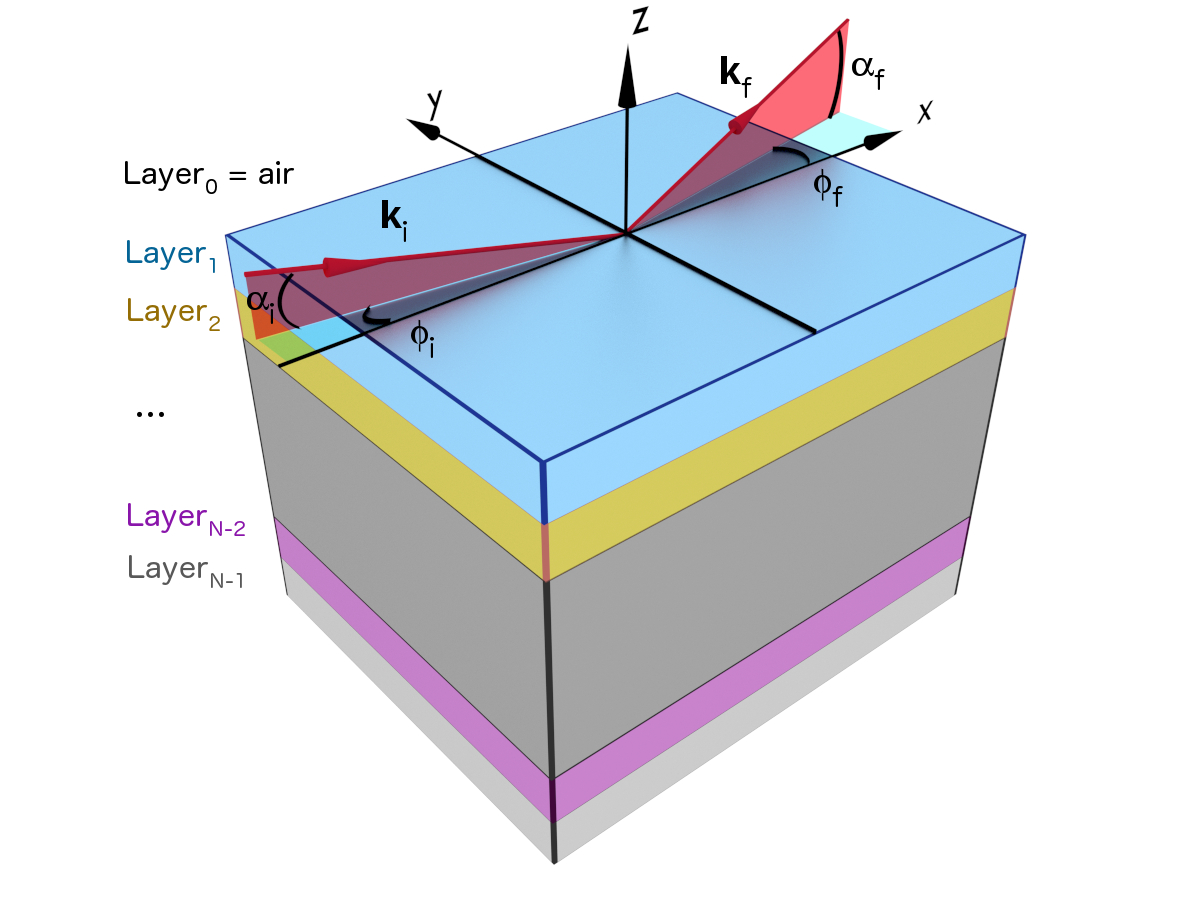
\includegraphics[clip=, width=120mm]{fig/drawing/setup_multilayer.jpg}
  \caption[Conventional GISAS scattering geometry.]{Geometric conventions
  in GISAS scattering comprise a Cartesian coordinate system
  and a set of angles.
  The coordinate system has a $z$ axis normal to the sample plane,
  and pointing into the halfspace where the beam comes from.
  The $x$ axis usually points along the incident beam,
  projected onto the sample plane.
  Incident and final plane waves are characterized
  by wavevectors $\k_\ti$, $\k_\tf$;
  the angle $\alpha_\ti$ is the incident glancing angle;
  $\phi_\ti$ is usually zero, unless used to describe a sample rotation;
  $\alpha_\tf$ is the exit angle with respect to the sample's surface;
  and $\phi_\tf$ is the scattering angle with respect to the scattering plane.
\nomenclature[1α024 2i000]{$\alpha_\ti$}{Glancing angle of the incident beam}
\nomenclature[1α024 2f000]{$\alpha_\tf$}{Glancing angle of the detected beam}
\nomenclature[1φ024 2i000]{$\phi_\ti$}{Angle between the incident beam, projected into the sample plane, and the $x$ axis}%
\nomenclature[1φ024 2f000]{$\phi_\tf$}{Angle between the detected beam, projected into the sample plane, and the $x$ axis}%
\nomenclature[2x020]{$x$}{Horizontal coordinate, usually chosen along the incoming beam projection}%
\nomenclature[2y020]{$y$}{Horizontal oordinate, chosen normal to $z$ and $x$}%
  The numbered layers illustrate a multilayer system as dicussed
  in Sect.~\ref{sec:Multilayers}.
  }
  \label{fig:expgeom}
\end{figure}

Reflectometry and grazing-incidence scattering
are designed for the investigation of surfaces, interfaces, and thin layers,
or most generically:
samples with a $2+1$ dimensional structure
that are on average translationally invariant in $x$ and $y$ direction,
but structured in $z$ direction.
By convention,
we designate the \textit{sample plane} ($xy$) as \textit{horizontal},
\index{Sample plane}%
\index{Horizontal plane}%
and the \textit{sample normal} ($z$) as \textit{vertical},
\index{Sample normal}%
\index{Vertical direction}%
even if this does not correspond to the actual experimental geometry.\footnote
{In many reflectometers,
 the scattering plane and the sample normal are horizontal in laboratory space.}
The $z$ axis points upwards, hence out of the sample towards the
vacuum (or air) halfspace where the incident radiation comes from,
as illustrated in Fig.~\ref{fig:expgeom}.
% TODO: add figure

Vertical modulations of the refractive index $n(\r)$
cause refraction and reflection of an incident plane wave.
\index{Glancing angle}%
\index{Refraction}%
\index{Reflection}%
For small glancing angles,
these distortions can be arbitrary large,
up to the limiting case of total reflection,
even though $1-n$ is only of the order $10^{-5}$ or smaller.
Such zeroth-order effects cannot be accounted for
by perturbative scattering theory.
Instead, we need to deal with refraction and reflection
at the level of the wave propagation equation.
We move the vertical variations of the squared refractive index
to the left-hand side of the Schrödinger equation~(\ref{EnSchrodi}),
\begin{equation}\label{EHelmholtzGraded}
  \left\{\Nabla^2+K^2\nz(z)\right\}\psi(\r)
  = 4\pi \chi(\r) \psi(\r),
\end{equation}
\nomenclature[2z020]{$z$}{Vertical coordinate, along the sample normal)}%
\nomenclature[2n030 2z020]{$\nz(z)$}{Refractive index, horizontally averaged}%
where the overline indicates an horizontal average.
Deviating from (\ref{EChiDef}),
the perturbation has been redefined as
\begin{equation}\label{EChiGraded}
  \chi(\r) \coloneqq  \frac{K^2}{4\pi}\left(\nz(z)-n^2(\r)\right),
\end{equation}
which only accounts for horizontal fluctuations of the refractive index.
Wave propagation,
unperturbed by~$\chi$, but including refraction and reflection effects,
obeys the homogeneous equation
\begin{equation}\label{EHelmholtzGradedHomog}
  \left\{\Nabla^2+K^2\nz(z)\right\}\psi(\r) = 0.
\end{equation}
It is solved for the horizontal coordinate~$\r_\parallel$
by the factorization ansatz
\Emph{
\begin{equation}\label{Ekpar}
\psi(\r) = \e^{i \k_\parallel\r_\parallel} \phi(z).
\end{equation}\vspace*{-10pt}
}
\nomenclature[2k041\parallel]{$\k_\parallel$}{Projection of $\k$ onto the sample plane}%
\nomenclature[1φ020 0z020]{$\phi(z)$}{$z$-dependent factor of $\psi(\r)$}%
The horizontal wavevector $\k_\parallel$ remains constant
as initialized by the incoming beam.
The vertical wavefunction must fulfill
\Emph{
\begin{equation}\label{Ewavez}
\left\{\partial_z^2 + K^2\nz(z) - k_\parallel^2 \right\} \phi(z) = 0.
\end{equation}\vspace*{-10pt}
}
When an incident plane wave,
travelling downwards with
$\phi(z)=\e^{-ik_\perp z}$,
\nomenclature[2k021\perp]{$k_\perp$}{Component of $\k$ along the sample normal}%
impinges on a sample with $\nz(z)\ne 1$,
then the wave is partly reflected ($-k_\perp$ reversed into $+k_\perp$)
and partly refracted
($k_\perp$ changing while $\k_\parallel$ stays constant,
resulting in a change of glancing angle).
Similarly, reflection and refraction occur
whenever $\nz(z)$ varies within the sample.
As a result, at any $z$ within the zone where $\nz(z)$ varies,
the vertical wavefunction $\phi(z)$ is composed of a
downward travelling component $\phi^-(z)$
and an upward travelling component $\phi^+(z)$.

For a graded refractive index
\index{Refractive index!graded}%
$\nz$ that is a smooth function of~$z$,
the differential equation~(\ref{Ewavez}) is best solved
using the WKB method.\footnote
{Also called \textit{semiclassical approximation} or
\textit{phase integral method},
%originally developed
%by Liouville (1837), Green (1837), Lord Rayleigh (1912), and Jeffreys (1923),
named after Wentzel (1926), Kramers (1926), Brillouin (1926).
See any textbook on quantum mechanics.}
\index{WKB method}%
\index{Semiclassical approximation|see {WKB method}}%
\index{Phase integral method|see {WKB method}}%
If otherwise $\nz(z)$ is discontinuous at some interface $z=z_j$,
then the limiting values of $\phi^-(z)$ and $\phi^+(z)$
on approaching $z_j$ from above or below
are connected to each other through Fresnel's
transmission and reflection coefficients.
\index{Fresnel coefficients}%
This applies in particular to multilayer systems,
discussed in chapter~\ref{sec:Multilayers}.

%===============================================================================
\subsection{Distorted-wave Born approximation (DWBA)}\label{SDWBA}
%===============================================================================

\index{Distorted-wave Born approximation|(}%
\index{DWBA|see {Distorted-wave Born approximation}}%

The standard form of the Born approximation,
as presented in Sect.~\ref{SBorn},
combines an approximation scheme
(computing (\ref{EPsiFormal}) by iteration)
with an assumption (the incident field is a plane wave)
and an analytic result
(in far-field approximation,
the Green function of the Helmholtz equation is a plane wave
with respect to the locus of scattering).
These three elements must not necessarily go together.
We can apply the very same approximation scheme,
even if the incident field is not a plane wave,
but a \textit{distorted wave},
namely a superposition of downwards and upwards travelling plane waves,
as derived in the previous section.
This is the core idea
of the \textit{distorted-wave Born approximation} (DWBA).\footnote
{The distorted-wave Born approximation
was originally devised by Massey and Mott (ca 1933)
for collisions of charged particles.}
% Schiff (^3 1968, p 327) cites
% Mott, Massey, The Theory of Atomic Collisions, p 100, Oxford 1933;
% There are also several papers by Massey and Mott from about 1933.

To carry out this idea, we need to determine the Green function~$G$.
\index{Green function!vertically structured material}%
In Sect.~\ref{SBorn} we did so quite specifically
for a homogeneous material.
Computing~$G$ in closed form for a more generic wave equation
like~(\ref{EHelmholtzGradedHomog}) is far more difficult,
if not outright impossible.
Fortunately, this computation is not necessary,
and would be but wasted effort:
We do not need the full solution~$G(\r,\r')$,
but only its asymptotic far-field value $G(\rD,\r')$
at a detector position $\rD$.
\nomenclature[2r041 2d100]{$\rD$}{Position of the detector}%
Thanks to a \textit{source-detector reciprocity theorem}~(\ref{Ereci})
\index{Reciprocity}%
proven in Appendix~\ref{Sreci1},
we can compute this value
as
\begin{equation}\label{EreciDup}
  G(\rD,\r) = B(\r,\rD),
\end{equation}
\nomenclature[2b030 2r040 2r041]{$B(\r,\r')$}{Green function, adjoint of $G$}%
where~$B$ is the \textit{adjoint Green function}
that describes backward propagation from $\rD$ into the sample.

Outside the sample,
$B$ obeys the Helmholtz equation
with isolated inhomegeneity (\ref{EHelmholtzForGreen}),
and therefore has the far-field expansion~(\ref{EGreenFar}),
\index{Far-field approximation}%
\begin{equation}\label{EBFar}
  B_\text{far}(\r,\rD)
  =\frac{\e^{iKr_\text{D}}}{4\pi r_\text{D}}\e^{-i\k_\tf \r}.
\end{equation}
When this backward propagating plane waves impinges on the sample,
it undergoes reflection and refraction in exactly the same way as
the incident plane wave $\e^{i\k_\ti\r}$.
Therefore,
 (\ref{EBFar}) admits a generalization that also holds inside the sample:
\begin{equation}\label{EBFull}
  B_\text{far}(\r,\rD)
  = \frac{\e^{iKr_\text{D}}}{4\pi r_\text{D}}\psi^*_\tf(\r).
\end{equation}
Applying now the reciprocity theorem (\ref{EreciDup}),
we obtain
\begin{equation}\label{EGreenFarDWBA}
  G_\text{far}(\r,\r')
  = \frac{\e^{iKr}}{4\pi r}\psi^*_\tf(\r')
\end{equation}
which agrees literally with (\ref{EGreenFar}),
though $\psi_\tf$ is not any longer a plane wave.
Accordingly,
the scattered far-field is still given by (\ref{EsandwichC}),
and the differential cross section by (\ref{Exsection}).

Since both the incident
and the scattered distorted wavefunction
are composed of downward and upward propagating waves,
\begin{equation}\label{Epsipm}
  \psi_w(\r)
  = \psi^-_w(\r) + \psi^+_w(\r)\text{~for~}w\in\{\ti,\tf\},
\end{equation}
\nomenclature[2w010]{$w$}{An index that can take the values i (incident)
or f (final)}%
the matrix element (\ref{Etrama})
can be expanded into four terms,
\begin{equation}\label{Edwba4}
  \bra \psi_\tf|\chi|\psi_\ti\ket
  = \bra \psi^-_\tf|\chi|\psi^-_\ti\ket
  + \bra \psi^-_\tf|\chi|\psi^+_\ti\ket
  + \bra \psi^+_\tf|\chi|\psi^-_\ti\ket
  + \bra \psi^+_\tf|\chi|\psi^+_\ti\ket,
\end{equation}
\nomenclature[1ψ041 0\pm 2r040]{$\psi^\pm(\r)$}{Upward ($+$) or downward ($-$) propagating component of $\psi(\r)$}%
\nomenclature[0\pm]{$\pm$}{Upward ($+$) or downward ($-$) propagating}%
or in an obvious shorthand notation
\Emph{%
\begin{equation}\label{Edwba}
  \bra \psi_\tf|\chi|\psi_\ti\ket
  = \sum_{\pm_\tf} \sum_{\pm_\ti}
    \bra \psi^\pm_\tf|\chi|\psi^\pm_\ti\ket.
\end{equation}%
\vspace*{-5pt}}
This equation contains the essence of
the distorted-wave Born approximation
for small-angle scattering under grazing incidence,
and is the base for all scattering models implemented in \BornAgain.
Note that $\bra \psi_\tf|\chi|\psi_\ti\ket$
appears as a squared modulus
in the differential cross section~(\ref{Exsection}).
Therefore, the four terms of (\ref{Edwba}) can interfere with each other,
which adds to the complexity of GISAS patterns.

\index{Distorted-wave Born approximation|)}%


%%%%%%%%%%%%%%%%%%%%%%%%%%%%%%%%%%%%%%%%%%%%%%%%%%%%%%%%%%%%%%%%%%%%%%%%%%%%%%%%
\section{Coherence length}\label{Scoherlen}
%%%%%%%%%%%%%%%%%%%%%%%%%%%%%%%%%%%%%%%%%%%%%%%%%%%%%%%%%%%%%%%%%%%%%%%%%%%%%%%%

The matrix elements $\bra \psi^\pm_\tf|\chi|\psi^\pm_\ti\ket$
are given by three-dimensional integrals~(\ref{Etrama}),
\begin{equation}\label{Etrama3}
  \bra \psi_\tf^\pm|\chi|\psi_\ti^\pm\ket
  \coloneqq  \int\!\d^3r\, \psi^{\pm*}_\tf(\r)\chi(\r)\psi^\pm_\ti(\r).
\end{equation}
The integrand factor $\chi$ is zero for
the top vacuum (or air) layer as well as for the bottom substrate,
which is assumed to have a horizontally constant refractive index.
Hence the $z$ extension of the integral is effectively limited
to a finite interval.

On the other hand, the horizontal integration domain is infinite.
This is of course an idealization.
Obviously, physical integration limits are imposed by the finite
\textit{illuminated sample area}.\footnote
{For a given instrument setup,
the incoming beam illuminates a finite area~$A_\ti$ in the sample plane,
and similarly, scattered radiation is only detected if it originates
from an area~$A_\tf$ that can be determined
by tracing back rays from the detector
to their intersection with the sample plane.
In a well aligned instrument, $A_\ti$ and $A_\tf$ are nearly the same.
Let $A_\text{beam}\coloneqq A_\ti\cap A_\tf$.
In a well aligned experiment,
$A_\text{beam}$ is equal to or a subset of $A_\text{sample}$
(if $A_\ti$ or $A_\tf$ are larger than $A_\text{sample}$,
collimation slits should be narrowed
lest useless rays cause avoidable noise).
Anyhow, the horizontal integration domain
is limited to the \textit{illuminated sample area}
$A_{xy}\coloneqq A_\text{sample}\cap A_\text{beam}$.}
\index{Sample area}%
\index{Illumination}%
Another limitation comes from the finite \textit{coherence length}
of the instrumental setup.
\index{Coherence length}%
This is of importance in neutron scattering
where typical sample dimensions of 1\ldots10~mm
are much larger than the relevant coherence length,
which is of the order 10\ldots100~$\upmu$m \cite{HaPR10,MaMM14}.\footnote
{These two references also make clear that
  the theoretical description and the experimental determination of
  coherence lengths are difficult problems and subject of ongoing research.}
The contrary is true for the scattering of synchrotron radiation,
where the coherence length typically exceeds the illuminated sample.

In contrast to synchrotron light,
a neutron beam is completely incoherent in the sense
that there are no interference effects between different neutrons.
While each single neutron is described by a wavefunction
that allows for \textit{coherent} superposition of
different scattering contributions,
the final detector statistics
\index{Detector statistics}%
is given by an \textit{incoherent} sum
over the differential cross sections of individual neutrons.
The finite \textit{resolution}
\index{Resolution|(}%
of an experimental setup is in part due to the fact that
different neutrons have different wavenumbers,
originate\footnote
{It is reasonable to take the last collision in the moderator
  as the \textit{origin} of a neutron ray,
  since collisions between neutrons and hydrogen nuclei bound in
  disordered matter lead to almost perfect decoherence.}
at different points in the moderator,
and are detected at slightly different points within one detector pixel.
This can be modelled by computing expected scattering intensities as
averages over different neutrons with 
$K$, $\v{\hat k}_\ti$, and $\v{\hat k}_\tf$ drawn at random
from appropriate distributions.

However, this is not the full story.
In the above introduction to the Born approximation
we have made the standard assumption
that an incoming neutron can be described by a plane wave
$\psi_\ti=\e^{i\k_\ti\r}$.
The wavefunction $\psi_\tf$ traced back from the detector is also
approximated by a plane wave.
In the DWBA we allow these waves to be distorted within the sample,
but when impinging on the sample they still are plane.
A plane wave obviously is an idealized concept,
since it has infinite lateral extension.
The \textit{transverse coherence length} indicates the scale
beyond which this approximation becomes invalid.
At larger scales, the wave fonts appear randomly distorted.
Physical causes of these distortions include
reflections in the neutron guide,
diffraction by guide windows and other slits,
and diffraction by imperfect monochromator crystals.
Of course the distorted wave still admits a Fourier decomposition
into plane waves with slightly different wavevectors.
In practice, it is impossibly to distinguish this spread of wavevectors
from the incoherent spread described in the previous paragraph.
The instrumental resolution function therefore
accounts for both causes of wavevector distortion.
\index{Resolution|)}%

Usually, therefore, a GISANS image is an incoherent average
over coherent diffraction patterns collected from 
many small subareas of the sample.
Only horizontal sample structures on scales smaller the coherence length
yield interference patterns.
Structure fluctuations on larger scales
produce said incoherent average of different GISANS images.

The crossover from coherent to incoherent scattering is of course
a gradual one.
The coherence length, however defined,
indicates where a certain, somewhat arbitrary degree
of decoherence is reached.
Under these reservations
one define a \textit{coherence spot}
in the cross section of an approximately plane wave
as an area where the coherence is above a certain threshold.
Unless the wave has been prepared in a highly anisotropic guide and slit system,
this spot is about circular.
Under grazing incidence conditions however,
the projection of this spot onto the sample surface
yields a very elongated ellipse.
Therefore, the coherence length is much larger in $x$ than
in $y$ or $z$ direction.\footnote
{This has nothing to do with the distinction of
  \textit{transverse} and \textit{longitudinal} coherence length.
  Longitudinal coherence has to do with wavelength stability
  and is of no importance for elastic scattering.
  We are talking here about \textit{horizontal} and \textit{vertical}
  projections of the \textit{transverse} coherence length.}

%%%%%%%%%%%%%%%%%%%%%%%%%%%%%%%%%%%%%%%%%%%%%%%%%%%%%%%%%%%%%%%%%%%%%%%%%%%%%%%%
\section{Absorption}\label{Sabsorption}
%%%%%%%%%%%%%%%%%%%%%%%%%%%%%%%%%%%%%%%%%%%%%%%%%%%%%%%%%%%%%%%%%%%%%%%%%%%%%%%%

\index{Refractive index!sign convention}%
The complex refractive index of a given material
shall be written as
\begin{equation}\label{Endb1}
  n\doteq 1-\delta +i\beta,  
\end{equation}
\nomenclature[1δ020]{$\delta$}{Small parameter in the refractive index
   $n=1-\delta +i\beta$}%
\nomenclature[1β020]{$\beta$}{Imaginary part of the refractive index}%
introducing two small real parameters $\delta, \beta$.
However, 
in our derivations, which are all rooted in~(\ref{EnSchrodi}),
$n$ only appears as $n^2$. 
Therefore, we actually \textit{define}
\begin{equation}\label{Endb2}
  n^2\coloneqq 1-2\delta+2i\beta,
\end{equation}
and read (\ref{Endb1}) as an excellent approximation.

While the real part of $n$ is responsible for refraction, reflection,
and scattering,
the imaginary part describes absorption
and leads to a damping of propagating waves.
The plus sign in front of the imaginary part is a consequence of
the quantum-mechanical sign convention;
in the X-ray crystallography convention it would be a minus sign.
\index{Sign convention}%

The factorization ansatz (\ref{Ekpar}) leaves us some freedom
how to deal with an imaginary part of~$n$.
We \textit{choose} that horizontal wavevectors $\k_\parallel$
shall always be real.
The damping then appears in the vertical wavefunction~$\phi(z)$
that is governed by the complex wave equation (\ref{Ewavez}).
